\documentclass{report}
\usepackage{graphicx}
\usepackage{booktabs}
\usepackage{amsmath,amssymb}
\usepackage{float}
\renewcommand{\thesection}{\arabic{section}}

\author{Trinh Thanh Vinh}
\title{Labwork 6: Map}

\begin{document}
\maketitle

\section{Introduction}
This labwork is about using CUDA map pattern for image processing. The same function is applied to every pixel of the image. All the pixels are processed in parallel. Three programs were implemented: grayscale binarization, brightness control, and image blending.

\section{Implementation}
First, image is loaded as an 8-bit value array. The array is then copied to the GPU, and a 2D CUDA grid is created. Each thread calculated its pixel position $(x,y)$ and checked that the position was inside the image. The grid size is also calculated to make sure the program works for any image size.

\subsection{Grayscale Binarization}
For every pixel, the kernel calculated the gray value from the average of the red, green, and blue channels. It then compared this value with a threshold. If the value is smaller than the threshold, the pixel is set to 0 (black); otherwise, it is set to 1 (white). The threshold can be adjusted to achieve different results, and it must be in the range of 0 to 255. The result is clamped to the range of 0 to 1.
\begin{figure}[H]
    \centering
    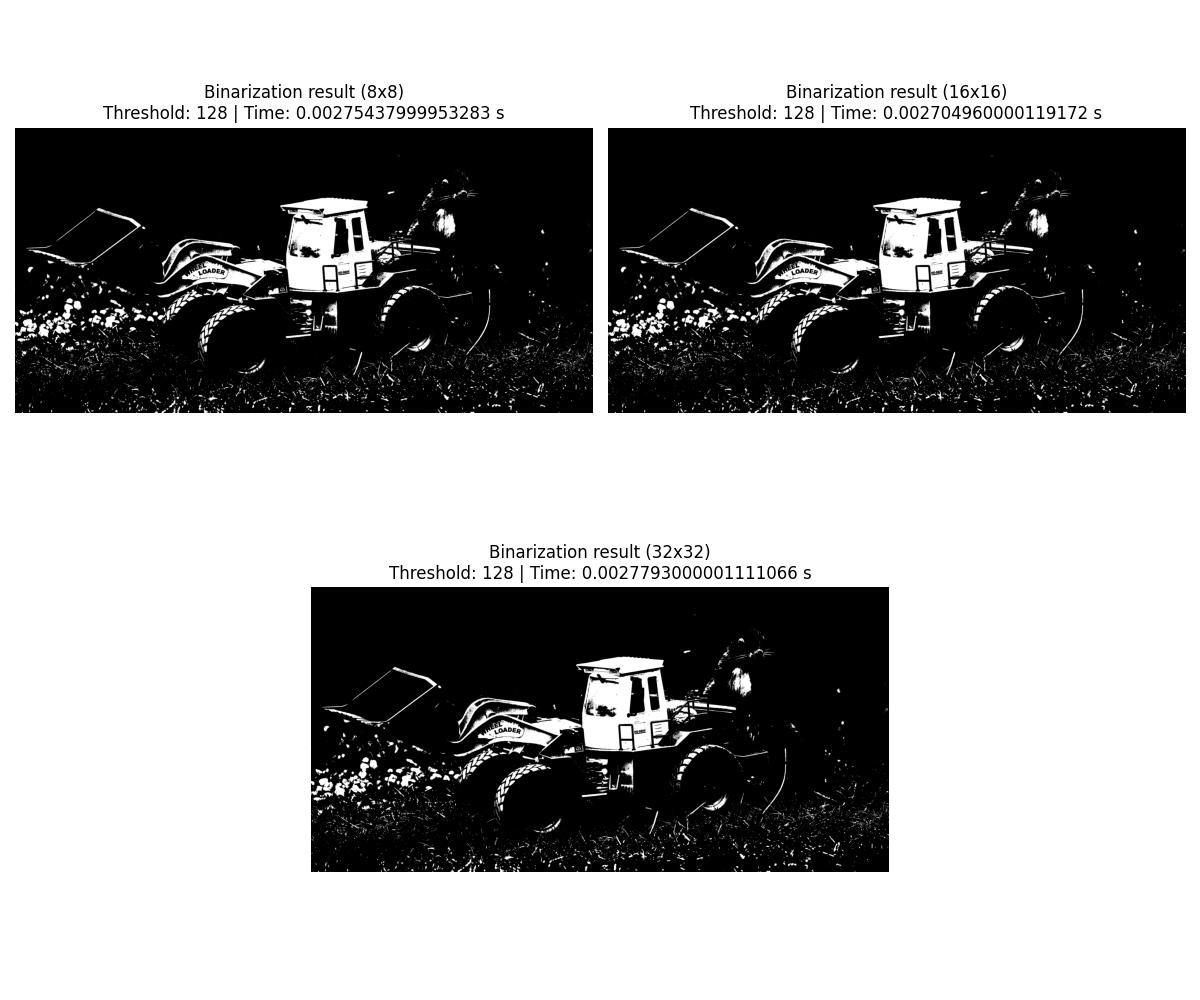
\includegraphics[width=0.50\linewidth]{binarization_results.jpg}
    \caption{Binarization results with three block sizes.}
\end{figure}

\subsection{Brightness Control}
The kernel added a positive or negative value, ranged from -255 to 255, to every RGB channels. Negative values darken the image, while positive values brighten it. The result is clamped to the range of 0 to 255 to avoid overflow or underflow.
\begin{figure}[H]
    \centering
    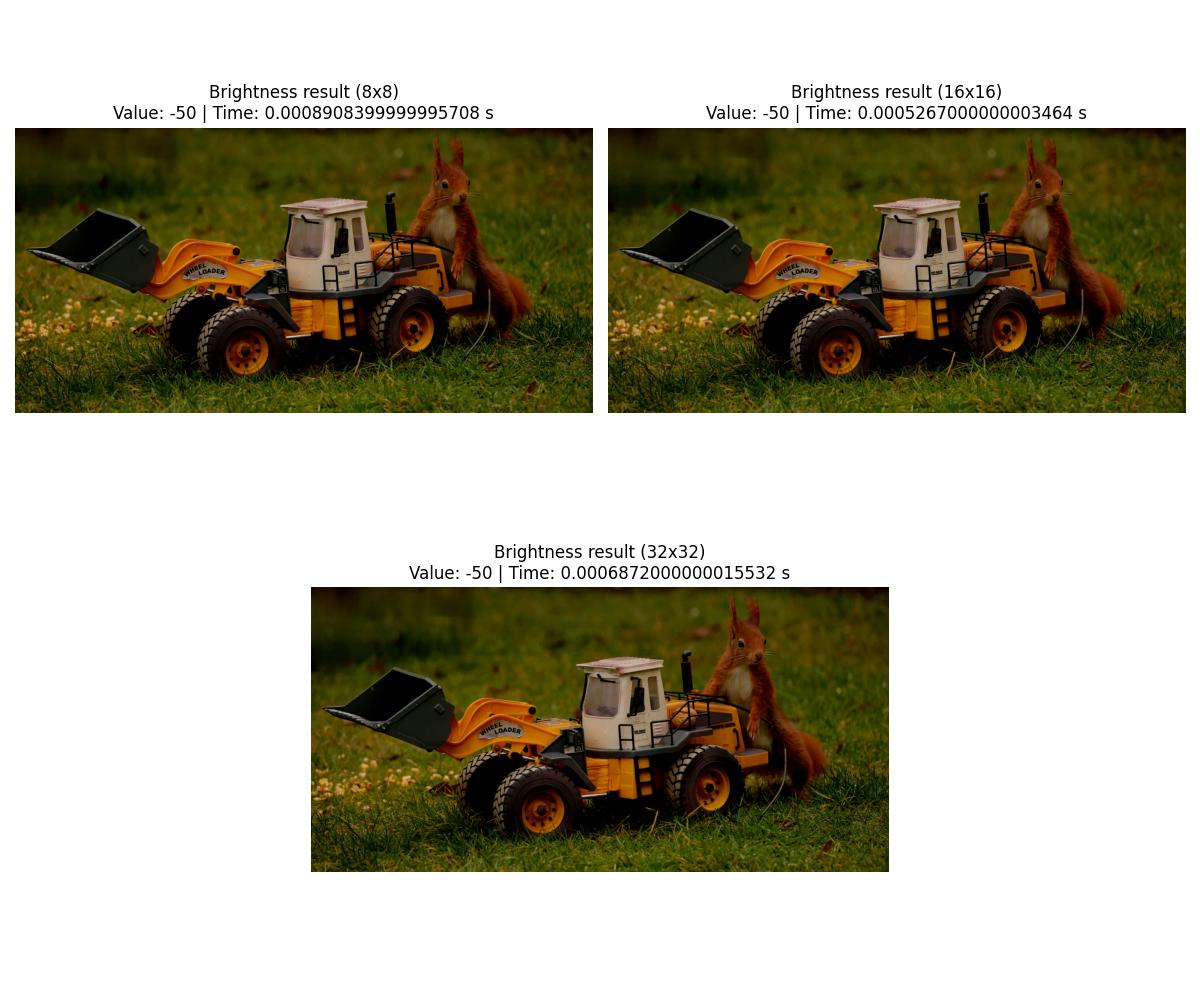
\includegraphics[width=0.50\linewidth]{brightness_results.jpg}
    \caption{Brightness results with three block sizes.}
\end{figure}

\subsection{Image Blending}
Two images with the same size are the input for this program. This is achieved by calculating a weighted average for each color channel. The weight is a value between 0 and 1, which can be adjusted to achieve different results. The result is clamped to the range of 0 to 255.
\begin{figure}[H]
    \centering
    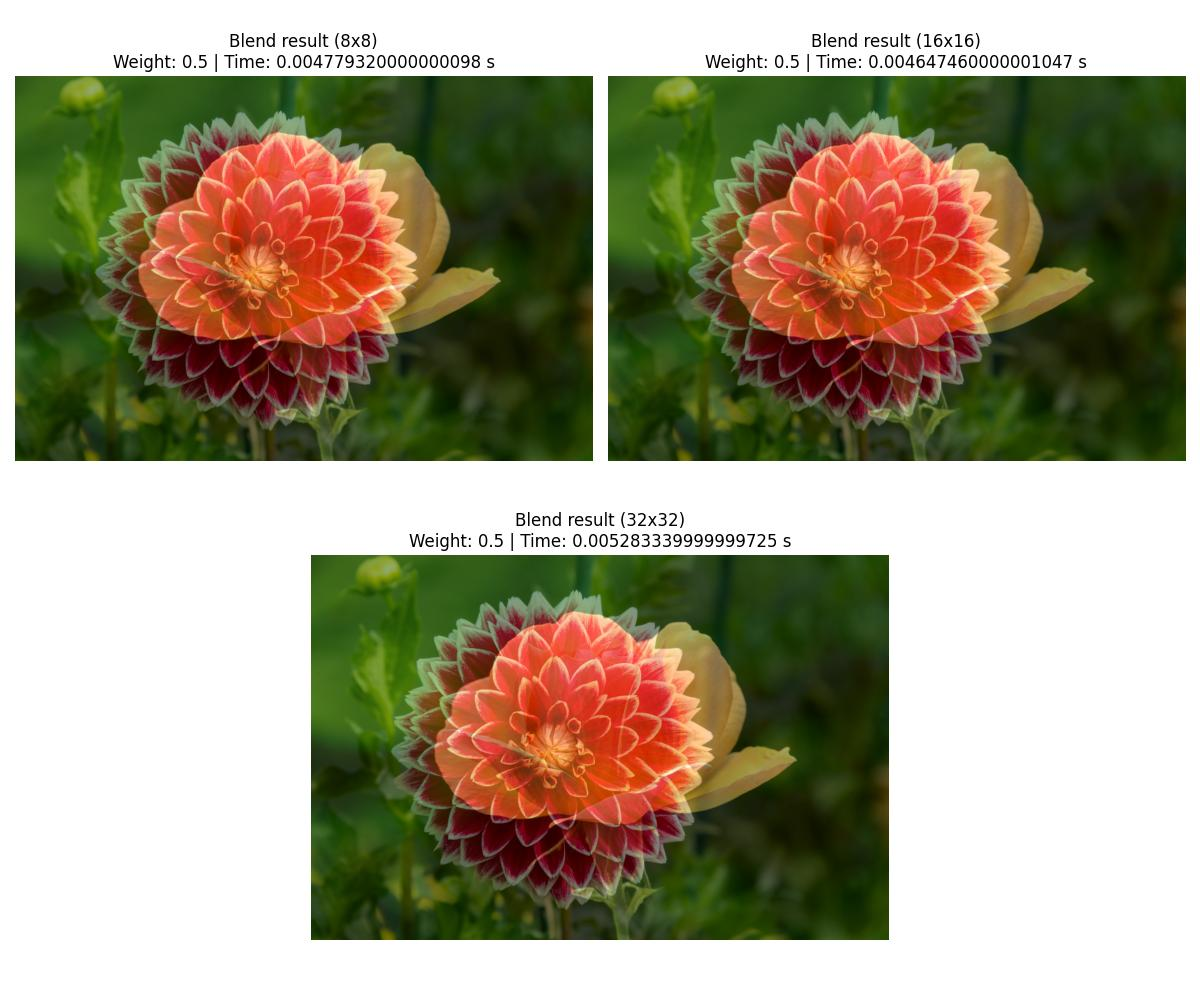
\includegraphics[width=0.50\linewidth]{blend_results.jpg}
    \caption{Blending results with three block sizes.}
\end{figure}

\section{Results}
The block sizes $8\times8$, $16\times16$, and $32\times32$ were tested. Before measuring, the kernel ran once as a warm-up. Each reported time is the average of five kernel runs. Data transfer time was not included.
\begin{table}[H]
    \centering
    \caption{Average GPU kernel time in milliseconds.}
    \begin{tabular}{|l|c|c|c|}
        \hline
        Operation & $8\times8$ & $16\times16$ & $32\times32$ \\
        \hline
        Binarization & 2.754 & 2.705 & 2.779 \\
        Brightness   & 0.891 & 0.527 & 0.687 \\
        Blending     & 4.779 & 4.647 & 5.283 \\
        \hline
    \end{tabular}
\end{table}
The
$16\times16$ block size was the fastest in all three tests. It gave a good balance between the number of threads in a block and the number of blocks. The differences were small, so the exact times can change with the GPU and the current computer load.
\end{document}